This chapter describes the search for a neutral MSSM Higgs boson decaying to a pair of $tau$. The studied final state is defined by the presence of a pair of reconstructed hadronic tau decays, this channel is thus named \tauh\tauh. The Standard Model Higgs boson decay into a pair of $tau$ leptons has been discovered by both the CMS and ATLAS collaborations \cite{ATLASHtt,CMSHtt}. In the context of the MSSM, three neutral Higgs bosons are predicted: the CP-even states h and H and the CP-odd state A, which may all decay to $\tau$ pairs. A model-independant search for a single Higgs boson, denoted $\Phi$, is performed with the free parameter $m_A$ in the range of $90$ to $3200\,\mathrm{GeV}$. The analysis is sensitive to production via gluon-gluon fusion and production in association with b-quarks. The cross section of the latter increases for larger values of $\mathrm{tan}\beta$ due to the enhanced down-type fermion Yukawa couplings.  %The search is also performed in the $m_A - \mathrm{tan}\beta$ parameter space of the $m_{h}^{max}$ scenario \cite{Carena2003} for the same mass range.

Similar searches for MSSM neutral Higgs bosons have previously been performed by the collaborations at LEP \cite{Schael2006}, the Tevatron \cite{Benjamin:2010xb}, and at LHC by the CMS and ATLAS collaborations \cite{Aaboud2018,Sirunyan2018} with no excess observed above the background expectation. 

The results presented here follow those published by CMS in 2018 using 2016 data, but makes use of the new 2017 data for the first time while being restricted to the \tauh\tauh channel. The 2017 data corresponds to an integrated luminosity of 41,5 $\mathrm{fb^{-1}}$. Event categorisation is used to enhance sensitivity to particular production modes. The production of neutrinos in the tau decays makes it difficult to reconstruct the invariant mass of the candidate Higgs boson. Statistical inference is therefore performed on the distribution of the \mttot variable, designed to give a better signal to background separation from the presence of neutrinos, and therefore \MET in signal events.

Section \ref{sec:analysis_samples} outlines the datasets of recorded collisions, defined by which trigger those collisions fired, and the simulation used to estimate certain backgrounds, which datasets are defined by the hard process used at generation. The event selection is then detailed in section \ref{sec:analysis_eventsel} which is done in a framework partially developed for this purpose. The estimation of each background process, using data-driven methods where possible, is detailed in section \ref{sec:analysis_background_methods} and followed by a summary of the experimental and theoretical uncertainties affecting the signal and background estimations in section \ref{sec:analysis_systematics}. The statistical procedure used to quantify the presence of signal in the data is given in section \ref{sec:analysis_statistical_interpretation} and is followed by the results of the search in section \ref{sec:analysis_results}.

\section{Data samples and simulation}
\label{sec:analysis_samples}

\subsection{Data triggers}
Collision datasets are defined by the trigger pattern that fired their recording. Events are therefore already selected at the L1 trigger level by an algorithm requiring either one L1-\tauh of $\pt > 70\,\mathrm{GeV}$ and $|\eta| < 2.1$, or two l1-\tauh of $\pt > 28\,\mathrm{GeV}$ and $|\eta| < 2.1$. At the HLT level, the di-\tauh triggers require two HLT-\tauh objects to be isolated, identified, to not overlap, and to each have $\pt > 35\,\mathrm{GeV}$ and $|\eta| < 2.1$. As stated in section \ref{sec:trigger}, these \tauh are reconstructed using a simplified version of the PF algorithm. Indeed, the object properties determined in the trigger reconstruction, such as \pt and isolation, are only approximate to those in the full reconstruction. Consequently, the triggering of events that could pass the offline event selection is not fully efficient. The trigger efficiencies for \tauh candidates typically reach $60\%$ at the lowest \pt threshold of the analysis, and reaches a plateau of between $85\%$ and $95\%$ at around twice the \pt thresholds \cite{Sirunyan_2018}. 

\subsection{Trigger optimisation}

In order to maximize the trigger efficiency for our analysis, asymmetric \pt threshold have been considered at the HLT level. The main concern of this study was finding a set of \pt thresholds that would gain efficiency while keeping the firing rate at the same magnitude. 
In order to estimate the efficiency gain, a new trigger pattern similar to the classical double \tauh trigger but without any \pt requirements was implemented. It was then applied to simulation of $H\rightarrow \tau\tau$ and DY $Z\rightarrow\tau\tau$ events. The \pt requirements on the trigger-level objects were then applied after the full reconstruction on the HLT level \tauh trigger objects to simulate the use of new \pt thresholds, and the efficiency was calculated as
\begin{equation}
    \epsilon = \frac{n_{\mathrm{trigger}}}{n_{\mathrm{selection}}} \mend
\end{equation}
In this expression, $n_{selection}$ is the number of events that pass the analysis requirements, and $n_{\mathrm{trigger}}$ is the number of these events that pass the trigger \pt requirements. This efficiency is then computed for different values of \pt requirements for each of the two \tauh trigger objects.

To estimate the firing rate in real collisions, the trigger pattern without \pt requirement was then applied to randomly selected collision events, to avoid pre-selection bias.  The rate were then computed from the random selection rate as
\begin{equation}
    f = \frac{n_{\mathrm{pass}}}{n_{\mathrm{total}}} \times f_{\mathrm{unbiased}} \mend
\end{equation}
In this expression, $n_{pass}$ is the number of events that pass the trigger threshold, $n_{total}$ is the total number of events of the unbiased sample, and $\mathrm{f}_{\mathrm{unbiased}}$ is the rate of random selection used to produce the unbiased sample. 

TODO: add the TH2 (maybe 2?)

While this study showed a gain of up to $6\%$ in efficiency through the use of asymmetric trigger thresholds, a $Z\rightarrow \tau\tau$ polarisation analysis showed the use of such a trigger pattern could reduce their acceptance of about $20\%$. The use of asymmetric \tauh trigger \pt threshold was therefore not implemented by the CMS collaboration.

\subsection{Simulation}
In the analysis, several MC generators are employed to produce simulated samples of signal and background events. The MADGRAPH \cite{Alwall2011} matrix element generator is used for Z+jets, W+jets, $\mathrm{t\Bar{t}}$+jets and diboson production. To increase the number of simulated Z+jets and W+jets events passing the most signal-sensitive category selections, additional samples are generated with fixed jet multiplicity in the matrix element for up to four jets. These are combined with the inclusive samples by weighting events to maintain the cross-section ratios between jet multiplicity bins. The POWHEG \cite{Alioli2010} generator is used for single top-quark production. The SM gluon-gluon fusion and VBF production modes of the Higgs boson, treated as a background in this analysis, are also simulated with POWHEG at NLO precision. Both $ggH$ and $bbH$ MSSM signal production modes are provided by PYTHIA \cite{SJOSTRAND2008852}. All samples utilise PYTHIA for parton showering and hadronisation, and TAUOLA \cite{JADACH1991275} for tau decays.


\section{Analysis sequence}
\label{sec:analysis_eventsel}

This section describes the event-based analysis sequence, which goal is to select, correct and derives quantities such as weights and physical variables like \mttot, the final discriminating variable defined as 
\begin{equation}
    \mttot = \sqrt{m_{T}^2(\tauh^{(1)},\MET) + m_{T}^2(\tauh^{(2)},\MET) + m_{T}^2(\tauh^{(1)},\tauh^{(2)})}
\end{equation}
where
\begin{equation}
    m_T (x,y) = \sqrt{2\times \pt^x \times \pt^y \times (1-\mathrm{cos}(\Delta \phi_{x,y}))} \mend
\end{equation}
First, we will provide an overview of the framework partially developed and used for this analysis, called heppy. This will be followed by a description of the analysis sequence.

\begin{figure}
    \centering
    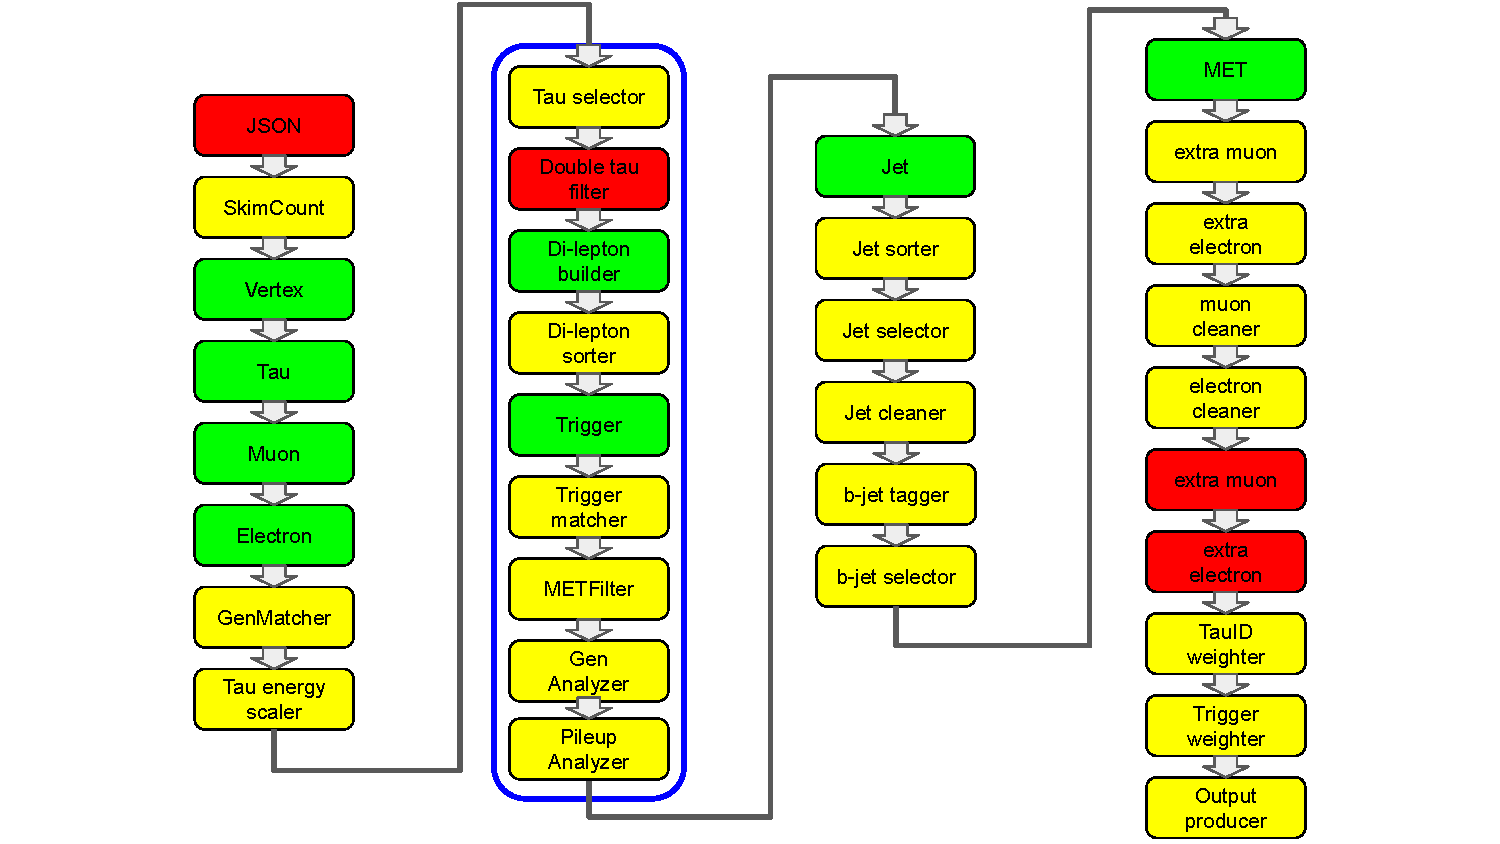
\includegraphics[width=\textwidth]{Images/HEPPY_diagram.pdf}
    \caption{Diagram of the selection flow implemented in heppy. Every box represents a module, called analyzer. Green analyzers create collections in the event instance by wrapping objects from the input in dedicated python classes. Yellow analyzers modify or compute a variable of the event. Red analyzers reject events that do not match given selection criteria. Finally, the blue highlighted section is the only part of the sequence that is specific to the $\tauh\tauh$ channel. The rest of the sequence is used in other channels, like the semileptonic channels $e\tauh$ and $\mu\tauh$, and has been successfully tested.}
    \label{fig:HEPPY}
\end{figure}

Heppy is a python event processing framework for high energy physics based on ROOT. The inputs used in this analysis follow the MINIAOD format of the CMS collaboration. This format was design to hold the event-based information needed by most analyses. Therefore, the input files hold a lot of information, i.e. the lists of reconstructed physics objects, making it quite important in size, leading to sizeable computing times. Events are first selected along the criteria defined in this section, while also trimming the information that is not useful to the analysis, leading to a new light-weight format. 

Heppy is a modular framework, which means all the processing is done in a feed-forward workflow with each step being encoded into a module called analyzer. Physics objects retrieved from the ROOT files are wrapped in python classes, allowing definition of useful methods and compatibilities. Most analyzer of this workflow manipulate the defined physics objects to either create new useful variables, select subsets or reject events based on specific criteria. New sets of analyzers have been created in order to provide as much modularity and clarity as possible so that equivalent stages of future analyses will be able to easily and promptly be implemented.

This section is focused on the desciption of the sequence for the \tauh\tauh channel. This sequence is applied to both simulation and real data, with some analyzer only being active in one of those cases. A diagram of the workflow developed is shown in figure \ref{fig:HEPPY}. In the order of use in the analysis flow, the role of the analyzers are the following:
\begin{itemize}
    \item JSON: Only active when running on real data. Rejects the events that have not been validated by the CMS collaboration.
    \item SkimCount: Only active when running on simulation. Counts the number of generated events before selection. This is used later to renormalize the number of generated events to match the data integrated luminosity.
    \item Vertex/Tau/Muon/Electron: creates collections of the respective objects, and adds useful methods and attributes to these objects.
    \item Gen matcher: Only active when running on simulation. Matches reconstructed \tauh with closest generator-level particles, and classify them following the scheme described in table \ref{tab:mc_matching}.
    \item Tau energy scaler: only active when running on simulation, scales the energy of \tauh, depending on their gen-level match. Stores each changes for later propagation to the \MET.
    \item Tau selector: first analyzer of the channel specific sequence, selects \tauh which have:
    \begin{itemize}
    \item $\pt > 40 \mathrm{GeV}$ and $|\eta| < 2.1$;
    \item passed the PF decay mode finding discriminator detailed in section \ref{sec:std_tau_id};
    \item $d_z < 0.2 \mathrm{cm}$, where $d_z$ is the displacement along the z-axis of the closest point of the leading charged track to the primary vertex;
    \item passed the very loose working point of the anti-electron discriminator and the loose working point of the anti-muon discriminator.
    \end{itemize}
    \item Double tau filter: Rejects the event if less than two \tauh fulfilling the requirements of the Tau selector have been found.
    \item Di-lepton builder: creates all possible combinations of two \tauh that have passed the selections, provided the \tauh:
    \begin{itemize}
    \item are separated by $\Delta R > 0.5$.
    \item have opposite-sign electric charges.
    \end{itemize}
    \item Di-lepton sorter: After these requirements, several pair of \tauh candidate can remain. In this case, the pair with the \tauh of highest \pt, called leading \tauh, is chosen. If two pairs have the same \pt for their leading \tauh, the pair with the most-isolated leading \tauh is chosen. In case of more than one pair with the same leading \tauh, the same criteria are then used on the second \tauh.
    \item Trigger: Retrieves the trigger information
    \item Trigger matcher: Checks if the selected \tauh pair matches with any of the L1 trigger patterns, and any of the HLT trigger patterns.
    \item MET Filter: Retrieves several flags that are provided by the CMS collaboration to reject events in order to mitigate several \MET reconstruction issues.
    \item Gen analyzer: Only active when running on simulation. Retrieves generator level information in order to compute several weights, i.e the top quark and Drell-Yan \pt reweighting that are detailed in the next section.
    \item Pileup analyzer: Only active when running on simulation, retrieves pileup information and computes pileup weights, as detailed in the next section.
    \item Jet: Creates collection of jets, and adds useful methods and attributes. Also applies the jet energy corrections as detailed in next section, while also storing the information for propagation to the \MET.
    \item Jet sorter: Sorts the jet collection by \pt.
    \item Jet selector: Jets are required to have $\pt > 30\,\mathrm{GeV}$ and $|\eta| < 4.7$, and to pass identification criteria to reject fake jets originating from detector noise, and pileup jets.
    \item Jet cleaner: Discards jets overlapping with one of the two selected leptons, i.e. distance between jets and any lepton must be $\Delta R > 0.5$.
    \item b-jet tagger: Applies a tag to each jet that defines if it is considered as a jet originating from a b-quark (b-tagged). The deepCSV method \cite{Sirunyan_2018} is used. Also applies b-tagging corrections as detailed in the next section.
    \item b-jet selector: Creates a b-tagged jet collection from all jets passing the b-tagging requirements defined in the b-jet tagger, and of $|\eta|<2.5$.
    \item MET: Retrieves \MET of the event. Applies all needed corrections detailed in the next section and adjust the \MET to compensate for all corrections applied to other physics objects.
    \item extra muon (electron) cleaners: Rejects events if any muons (electrons) passes a set of quality criteria, not considering the selected leptons when running on the semi-leptonic channels.
    \item TauID/trigger weighters: compute and apply the respective correction weights detailed in the next section.
    \item Output producer: Gathers all desired information and stores it in a flexible ROOT format allowing production of the distributions for statistical inference.
\end{itemize}

The output of this stage is used to perform a synchronisation with other CMS institutes working on the same analysis. For example a prototype of this sequence was used to synchronise on the previous MSSM search for a heavy Higgs bosons \cite{Aaboud2018} and helped figure out tweaks and upgrades in other group codes. For this 2017 data analysis, a new synchronisation has been successfully performed.


\section{Background estimation methods}
\label{sec:analysis_background_methods}

For all processes apart from QCD multijet events, appropriate samples of MC simulation are available. While most background will be estimated by data-driven methods, these simulated samples are still used for a small part of the background contributions. Data-driven techniques not only tend to improve the data/MC agreement but also reduces the involved systematic uncertainties. Section \ref{sec:embedding} details how embedded samples are used to estimate $\mathrm{Z} \rightarrow \tau\tau$ events with two genuine tau lepton decays involved. And section \ref{sec:ff} describes how events where at least one of the tau candidates is faked by a jet are estimated by the fake factor method.

Monte-carlo simulated events (MC) are meant to provide an estimation of the contribution of processes that are not covered by the data-driven techniques. The data-driven techniques cover contributions based on the \tauh decay provenance. To distinguish the relevant processes that must be estimated from simulation, the reconstructed \tauh have to be matched to the generator particles available in the simulated samples. This is called referred to as gen matching. The exact definitions used to distinguish the different matched types can be found in table \ref{tab:mc_matching}.

\begin{table}[]
    \centering
    \caption{MC generator matching.}
    \begin{tabular}{|c|c|l|}
        \hline
        Value & Type & Generator level object properties \\
        \hline
        \multirow{2}{*}{1} & \multirow{2}{*}{Prompt electron} & $|\mathrm{pdgID}|==11$, $\pt > 8 \,\mathrm{GeV}$,\\
         & &  status flag IsPrompt \\
        \hline
        \multirow{2}{*}{2} & \multirow{2}{*}{Prompt muon} & $|\mathrm{pdgID}|==13$, $\pt > 8 \,\mathrm{GeV}$, \\
         & & status flag IsPrompt \\
        \hline
        \multirow{2}{*}{3} & \multirow{2}{*}{$\tau \rightarrow e$} & $|\mathrm{pdgID}|==11$, $\pt > 8 \,\mathrm{GeV}$,\\
         & &  status flag IsDirectPromptTauDecayProduct \\
        \hline
        \multirow{2}{*}{4} & \multirow{2}{*}{$\tau \rightarrow \mu$} & $|\mathrm{pdgID}|==13$, $\pt > 8 \,\mathrm{GeV}$, \\
         & & status flag IsDirectPromptTauDecayProduct \\
        \hline
        \multirow{2}{*}{5} & \multirow{2}{*}{$\tau \rightarrow \tauh$} & \multirow{2}{*}{Gen-tau jet} \\
         & & \\
        \hline
        \multirow{2}{*}{6} & \multirow{2}{*}{Jet or pu fake}  & Anything that does not fall into \\
         & &  any of the above categories \\
        \hline
    \end{tabular}
    \label{tab:mc_matching}
\end{table}

The simulated background samples are split into three categories labeled T, J and L. T corresponds to events with gen match = 3, 4, 5 for both tau candidates. J corresponds to events with gen match = 6 for at least one of the hadronic tau candidates. L corresponds to all remaining events. In this analysis the T part of the background samples is replaced by the embedded samples and the J part is covered by the fake factor method. The remaining part is then covered by simulation.


\subsection{Monte-Carlo simulation}
\label{sec:MC_corr}

In order to mitigate the differences between data and simulations, several measurements have provided corrections that are applied in the analysis. These corrections are:

\paragraph{Pileup reweighting} MC simulated samples are generated with a given instantaneous luminosity which does not match the instantaneous luminosity of the data, which is often recorded after or during the production of the MC samples. In order to better fit the recorded pileup distribution in data a pileup reweighting is applied to MC events.

\paragraph{EE noise jets removal} Due to noise in the ECAL endcaps, all jets in a pseudo-rapidity gap of $2.65 < |\eta| < 3.139$ and of less than $50 \,\mathrm{GeV}$ are removed in both data and MC. The removal of the jet is also propagated to the \MET.

\paragraph{\tauh reconstruction efficiency} A data/MC scale factors (SF) is measured in $\mathrm{Z}\rightarrow\tau\tau$ events using a tag-and-probe approach. The selection of the tag-and-probe pairs is defined as follows. The tag \tauh must satisfy the kinematic, ID, and isolation requirements used in the analysis, in data it should also be matched to a trigger object. Probe leptons are only required to pass the kinematic cuts. Pairs of tag and probe leptons are considered when the leptons are same flavour and opposite sign charge, and are well separated ($\Delta R > 0.5$). The ID and isolation requirements used in the analysis are tested on the probe leptons, that can either pass or fail. The ID and isolation efficiency is defined as the number of passing probes divided by the total number of probes. The final efficiencies are extracted from a fit to the di-lepton invariant mass in the mass window around the $\mathrm{Z}$ mass. The scale factor applied to MC events is given by the ratio:
\begin{equation}
    SF = \frac{\epsilon(\mathrm{data})}{\epsilon(\mathrm{MC})} \mend
\end{equation}
For the embedded samples this scale factor is measured using a similar procedure. An additional correction is applied for embedded taus to correct for biases due to higher tracking efficiencies in embedded events than data. 

\paragraph{\tauh triggering efficiency} Trigger scale factors are also measured using a tag and probe method. For the trigger efficiency measurement, both the tag and the probe leptons must pass the ID and isolation requirements applied in the analysis, and passing probes are the ones firing the considered trigger. The efficiencies of the triggers are measured for data and MC. The scale factors for the double-\tauh trigger are measured in bins of the tau \pt, $\eta$, and $\phi$. Due to a bug in the embedded samples the efficiency of the tau triggers is significantly lower than the non-embedded SF. This bug affects some of the HLT requirements relating to the hadronic tau isolation cuts. To fix this issue the embedded taus are matched to earlier versions of the HLT \tauh objects before the problematic part. The scale factors are then used to cover the differences. The scale factors for the embedded samples use the same $\epsilon(\mathrm{data})$ measured for the MC scale factors but use the efficiency measured for the embedded taus in the denominator, the scale factor is then computed as:
\begin{equation}
    SF = \frac{\epsilon(\mathrm{data})}{\epsilon(\mathrm{embedding})} \mend
\end{equation}

\paragraph{Tau energy scale} The tau energy scale was measured using as observables the tau mass and the invariant mass of the system of the muon and the hadronic tau decay in $\mathrm{Z}\rightarrow\tau_{\mu}\tauh$ events. 

\paragraph{Jet energy} On top of the corrections detailed in section \ref{sec:jet_clustering}, corrections derived by the CMS collaborations to mitigate data/MC discrepencies are also applied \cite{collaboration_2011}.

\paragraph{Efficiency of lepton faking \tauh} Lepton can fake \tauh decay products, as their track can be misreconstructed as a charged hadron. The rates of such misreconstructions are measures by the collaboration and corrections are applied to simulation to match data expectation.

\paragraph{Lepton faking \tauh energy scale} A correction to the central values of the \tauh energies for \tauh candidates originating from electron (muon) fakes is applied for the 1-prong and 1-prong+1-\pizero decay-modes \cite{Chatrchyan2011}. 

\paragraph{Recoil corrections} Recoil corrections are applied to correct for the mismodeling of \MET in the simulated Drell-Yan, W+Jets and Higgs production. The corrections are measured on the vector $\Vec{U}$ defined as the vectorial difference of the measured missing transverse momentum and total transverse momentum of neutrinos originating from the decay of Z, W or Higgs boson
\begin{equation}
    \Vec{U} = \Vec{\MET} - \Vec{p}_{T,\nu} \mend
\end{equation}
The vector $\Vec{U}$ is projected onto the axes parallel ($U_1$) and orthogonal ($U_2$) to the boson \pt and it is measured in $\mathrm{Z}\rightarrow \mu\mu$ events, where the leptonic recoil does not contain neutrinos and the four-vector of the Z boson can be measured precisely. The effect of the recoil corrections on the \MET distribution of $\mathrm{Z}\rightarrow \mu\mu$ events, as measured by another CMS institute, is shown in figure \ref{fig:recoilcorr}.

\begin{figure}
\centering
\begin{subfigure}[b]{0.5\textwidth}
  \centering
  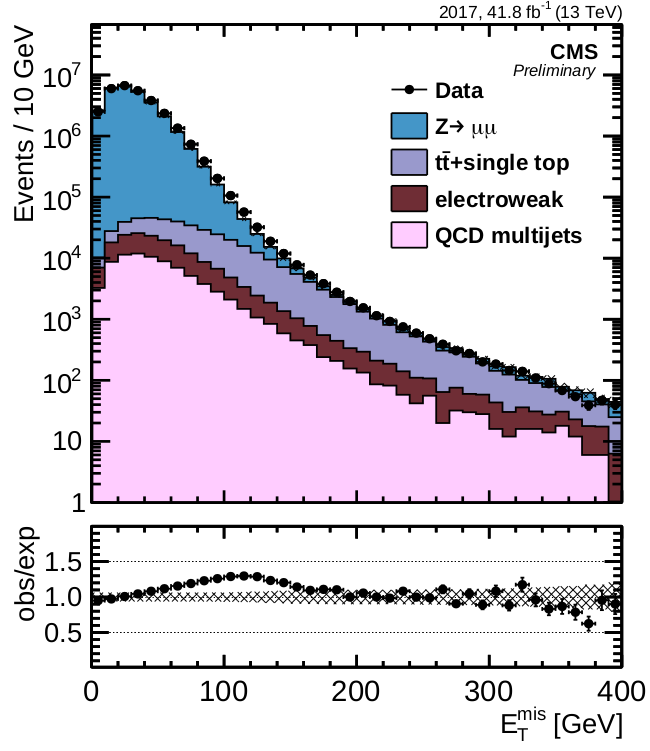
\includegraphics[width=\textwidth]{Images/withoutrecoil.png}
  \caption{\label{fig:recoil1} Without recoil corrections}
\end{subfigure}%
\begin{subfigure}[b]{0.5\textwidth}
  \centering
  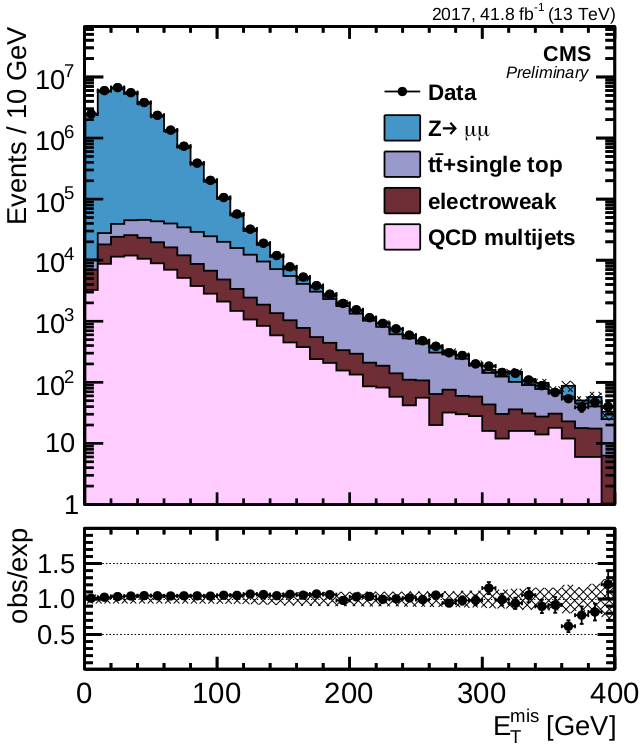
\includegraphics[width=\textwidth]{Images/withrecoil.png}
  \caption{\label{fig:recoil2} With recoil corrections}
\end{subfigure}
\caption{Effect of applying recoil corrections to the \MET distribution in the $\mathrm{Z}\rightarrow \mu\mu$ selection.}
\label{fig:recoilcorr}
\end{figure}

\paragraph{DY mass and transverse momentum reweighting} A reweighting is applied to Drell-Yan MC samples to correct the generator-level \pt and generator-level di-lepton mass distributions in LO madgraph samples. The correction is produced in a $\mathrm{Z}\rightarrow \mu\mu$ control region, as a function of the \pt of the $\mathrm{Z}$ and generator di-lepton mass to reduce the shape discrepancy between data and simulation. The weights are computed in such a way as to make the two-dimensional distributions of the $\mathrm{Z}$ \pt and the Z boson reconstructed mass match between data and simulation. The weights are then corrected not to introduce a general yield variation of the Drell-Yan background, but to only have a shape effect on the considered distributions. Those distributions before and after reweighting are shown in figure \ref{fig:DYreweight}.

\begin{figure}
    \centering
    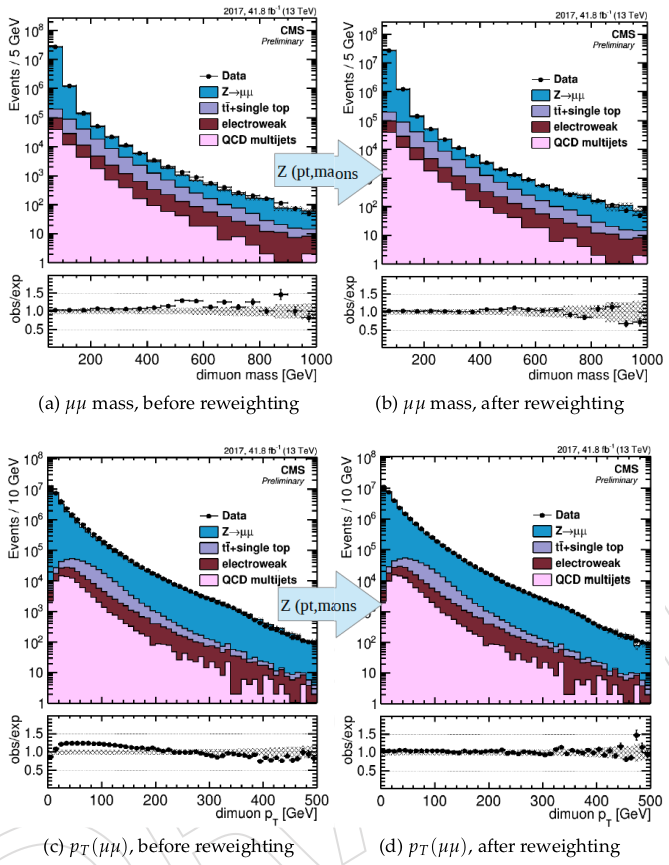
\includegraphics[width=.7\textwidth]{Images/DYreweight.png}
    \caption{Di-muon mass and \pt distributions in $\mathrm{Z}\rightarrow \mu\mu$ data before and after the reweighting.}
    \label{fig:DYreweight}
\end{figure}

\paragraph{Top quark transverse momentum reweighting} The modeling of the $t\Bar{t}$ background is improved by reweighting the \pt spectrum of the top quarks.

\paragraph{b-tagging efficiency} The efficiency for the tagging of b jets and the mistagging rate for light-flavour jets has been measured in both data and simulation. The efficiency and mistagging rate of the simulation is corrected through the application of efficiency and mistagging scale factors. The values of these factors and a description of the methods used to determine them can be found in \cite{Sirunyan_2018}. The simulation is corrected by randomly reclassifying, or demoting a fraction of tagged jets as untagged, or the other way around, i.e promoting, as necessary to result in the correct average efficiency and mistagging rate. The promotion or demotion probabilities for each jet are defined as
\begin{equation*}
    P(\mathrm{demote}) = 1 - SF \msep \text{when } SF < 1
\end{equation*}
\begin{equation*}
    P(\mathrm{promote}) = \frac{(SF-1)\epsilon}{\frac{SF}{\epsilon-1}} \msep \text{when } SF > 1 \mend
\end{equation*}
In this expression, the scale factor, $SF$, is $\pt$, $\eta$ and jet-flavour dependant ratios of data and simulation efficiencies, and $\epsilon$ is the measured tagging efficiency.

% \begin{figure}
%     \centering
%     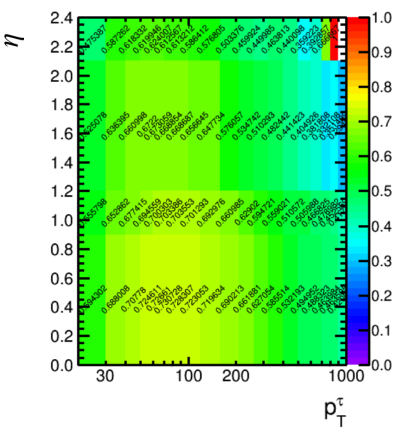
\includegraphics[width=.5\textwidth]{Images/btag_eff.png}
%     \caption{The b-tagging efficiency measured using $t\Bar{t}$ and DY MC in bins of b-jet $\eta$ and \pt.}
%     \label{fig:btageff}
% \end{figure}

\subsection{Embedding}
\label{sec:embedding}

The embedding technique allows an estimation of the standard model backgrounds with two taus in the final state from data, with minimal simulation input. A sample of di-muon events is selected from the recorded data. The two muons are removed from the event and replaced with simulated tau leptons with the same kinematic properties. In that way a set of hybrid events is obtained that relies on simulation only for the decay of the tau leptons. challenges in describing the underlying event or the production of associated jets in the simulation are avoided. A detailed description of the embedding technique can be found in \cite{CMS:2018apv}.

In this analysis, embedded samples are used in place of the MC simulated samples for $\mathrm{Z}\rightarrow \tau\tau$ and the parts of $t\Bar{t}$, di-boson and electroweak events where both tau candidates are matched to genuine taus at generator level.

\subsection{Fake factor method}
\label{sec:ff}
\begin{figure}
\centering
\begin{subfigure}[b]{0.5\textwidth}
  \centering
  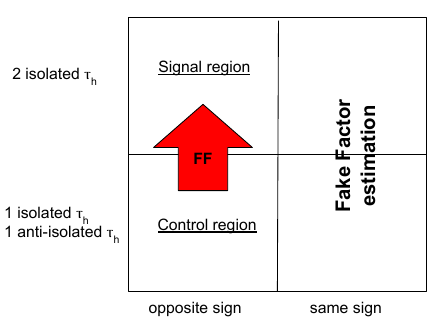
\includegraphics[width=\textwidth]{Images/FF_method.png}
  \caption{\label{fig:FF_method}}
\end{subfigure}%
\begin{subfigure}[b]{0.5\textwidth}
  \centering
  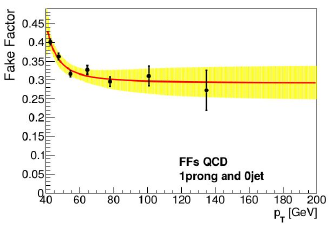
\includegraphics[width=\textwidth]{Images/FF_values.png}
  \caption{\label{fig:FF_values}}
\end{subfigure}
\caption{Illustration of the fake factor method. Diagram \subref{fig:FF_method} illustrate the way fake factors are measured, while \subref{fig:FF_values} illustrate some the values and fitted function used in the case of \tauh decaying to 1 prong and 0 jet in the event.}
\label{fig:FF_illustration}
\end{figure}

The fake factor method (FF) is used to predict all background sources with gluon- or quark-initiated jets misidentified as hadronic $\tau$ decays. The method is based on measuring the ratio of the number of events where preselected jets pass the \tauh ID criteria over the number of events that do not pass the ID criteria. Different regions are used to perform this measurement, depending on which background process is considered, namely QCD multi-jet, W+jets and $t\Bar{t}$. The preselection is defined by the same set of selection as the analysis, with the difference of a looser \tauh ID criteria, defining a region called the anti-isolated region. The value of the fake factor (FF) is then defined as
\begin{equation}
    FF = \frac{\text{passes preselection and passes \tauh ID discriminant}}{\text{passes preselection and fails \tauh ID discriminant}} \mend
\end{equation}
This fake factor is applied as a weight to events which pass the signal region selection except that the events are required to contain \tauh candidates satisfying the preselection criteria, but failing the nominal \tauh ID criteria (application region). The fake factor is estimated as a function of the jet multiplicity (0 or $\geq$ 1) and the \pt dependency is fit.

The fake factors are also determined separately for each of the channels $e\tauh$, $\mu\tauh$, and $\tauh\tauh$, accounting for differences in the selected background composition, the trigger requirements and in the \tauh ID criteria applied in each channel. For the \tauh\tauh channel, the determination region requirement is that the electric charges of the two hadronic $\tau$ candidates have the same sign. As for this channel the multi-jet background is by far the dominant fake \tauh background, the fake factors measured in the QCD determination region are also used to estimate any other backgrounds arising from fake \tauh.

The fake factor applied to a given event in the application region is a weighted average of the values measured for the different processes. The weight is given by the expected fraction of events of a given process in the application region. The weight is binned in $m_{vis}$ and number of jets. This weighted fake factor is applied to all events in the application region twice, once considering a \tauh as the fake, then considering the other as a fake, while multiplying both weights by $0.5$. Since genuine tau events in data are also present in the application region, the expected contribution from events with actual hadronic $\tau$ decays are subtracted using simulation. The expected fraction of events is estimated in two independent ways: via a template fit to the observed data, and via simulation. As the results of both methods agree and the template fit has convergence problems in some low-statistics event categories, the simulation-based estimate is used.

\section{Systematic uncertainties}
\label{sec:analysis_systematics}

This section describes the sources of uncertainty that affect the signal and background predictions of the \mttot distributions in each category. The experimental uncertainties typically concern either object selection or the methods to estimate the backgrounds described in the previous section, and are inherent to their respective measurement. The object selection is more important for the signal prediction, whereas the estimation methods have a large effect on the background estimation. Theoretical uncertainties affect the predictions of both signal and simulated background but are larger for the signal. Uncertainties can affect only the rate of signal, but some may affect both the shape and rate of the distributions. Each source of uncertainty will give a free parameter, called nuisance parameter, in the background estimation fit described in the next section.

\subsection{Shape uncertainties}

Most shape uncertainties, are evaluated by re-running the concerned simulated events through the workflow, but this time applying the up or down fluctuation on the considered variable. This leads to a multiplication of the overall computing needed to perform the full analysis, and is the main reason the semi-leptonic channels are not included in this analysis.

The following uncertainties cause variations in the shapes of the distributions.

\paragraph{Tau energy scale} Since the \mttot variable depends on the \pt of the selected \tauh, a separate shape uncertainty is applied for each decay mode in the simulated samples. In the embedded samples we have hybrid events where the simulated taus might be mixed with calorimeter deposits remaining from the removal of the original muons in the events. For this reason, the tau energy scale uncertainties for embedded samples are split into two parts, where $50\%$ are fully correlated with the uncertainty for fully simulated samples and $50\%$ are uncorrelated.

\paragraph{Jet energy scale} Since the change in jet energy is propagated to the \MET, the jet energy scale impacts the shape of the \mttot distribution. In general, the CMS collaboration derives uncertainties in the jet energy scale from 28 sources and combines them in a single uncertainty with one nuisance parameter. The uncertainty is split into several groups, instead of all 27 sources, because this would result in an unnecessary amount of parameters in the fit as well as a large technical effort. Instead, the sources are grouped according to the affected detector regions.

\paragraph{Energy scale of leptons faking \tauh} Shape uncertainties are applied to the \pt of the misidentified \tauh arising from the presence of leptons in MC samples uncorrelated between decay modes.

\paragraph{\MET unclustered energy uncertainty} The \MET takes into account the energy that is not clustered in the reconstruction process, impacting the value of \mttot. An uncertainty is therefore applied to all MC processes that do not have recoil correction applied.

\paragraph{\MET recoil correction uncertainties} For all MC processes that have recoil correction, uncertainties determined during the computation of the recoil corrections are propagated to the \mtot variable.

\paragraph{Top \pt reweighting} The uncertainty in the top \pt reweighting are estimated by not applying the correction and applying twice the correction in the $t\Bar{t}$ events.

\paragraph{DY \pt reweighting} The uncertainty in the DY \pt reweigthing are estimated by shifting of $10\%$ re-weighting applied to $\mathrm{Z}\rightarrow ll$ events.

\paragraph{B-tagging efficiency} The uncertainties in the b-tagging scale factors provided by the CMS collaboration are propagated to the the \mttot distribution in the categories defined by the presence or absence of b-tagged jets.

\paragraph{\tauh tracking efficiency for the embedded samples} An uncertainty in the tracking efficiency of hadronic taus in the embedded samples is propagated uncorrelated between 1 and 3 prong decay modes.

\paragraph{Fake-factor uncertainties} Uncertainties in the fake factor background estimation method consist of several sources:
\begin{itemize}
    \item Statistical uncertainty in the fake factor measurement in the control regions.
    \item Systematic uncertainties related to the QCD multi-jet fake factor corrections are propagated.
    \item Systematic uncertainties in the fraction of W/Z+jets events and $t\Bar{t}$ events with one misidentified \tauh in the anti-isolated region, adding two nuisance parameters. Those is evaluated by varying the fractions of those two background within uncertainties (including cross section and experimental uncertainties), while readjusting the fractions of the other processes to keep the sum at $100\%$.
\end{itemize}

\paragraph{Bin-by-bin uncertainties} To account for statistical shape uncertainties in the backgrounds due to the use of Monte-Carlo and embedded samples or templates derived from data events with limited number of events, we introduce shape variations to the background templates in all categories following the Barlow-Beeston approach, where the statistical uncertainties in each bin are used to define alternative shapes.

\subsection{Normalization uncertainties}

The number of events from each process is affected by a normalization uncertainty. A nuisance parameter following a log-normal distribution is applied on the yield of the affected process.

\paragraph{Luminosity} A $2.3 \%$ luminosity uncertainty is applied to the number of events predicted by pure Monte Carlo simulation \cite{CMS:2018elu}.

\paragraph{Tau ID efficiency} The uncertainty is applied to the number of events for all processes where the yield is estimated from MC, as well as the embedded events. Since two hadronic taus are required in the \tauh\tauh channel the magnitude of the uncertainty is $2.4\%$ for each \tauh, maning $5.5\%$ overall. The embedded samples also have an additional uncertainty applied to cover a tracking efficiency correction, with a magnitude of $2\%$ per \tauh.

\paragraph{Trigger efficiency} The uncertainty in the trigger efficiency amounts to $10\%$. The uncertainty is applied to all processes where the yield is estimated from MC, and to the embedded samples. The embedded and MC uncertainties are uncorrelated. In order to account for the efficiency of the double muon trigger that was used to select input events for the embedding technique, an additional $4\%$ uncertainty ($2\%$ per muon $= 4\%$) is applied to the embedded samples.

\paragraph{Background normalization uncertainty} A $4\%$, $5\%$, $6\%$ and $4\%$ uncertainty is applied to the $Z\rightarrow ll$, di-boson/single top, $t\Bar{t}$ and EWKZ processes, respectively, to account for the uncertainty in the production cross section of these processes. 

% \paragraph{Lepton to tau fake rate} Shape uncertainties were checked and no significant shape dependency has been observed in the event distributions used in this analysis. Therefore log normal uncertainties of $16\%$ ($26\%$) are applied for electron (muon) to tau fake rate.

\paragraph{Fake factor normalization} The uncertainty due to the subtraction of the genuine tau contribution is estimated by varying the substracted number of events by $\pm 10\%$, and amounts to about $2\%$ of the jet faking \tauh yield. %The fake factor shape uncertainties are normalized to the same area as the nominal shape, and the normalization factors are added in quadrature and act as separate nuisance parameters: this is done separately for the statistical uncertainties in the raw fake factors (about $5\%$) and the systematic uncertainties in the corrections (about $7\%$). Uncertainties are split in shape(-only) and yield uncertainties to capture the main variations induced by the uncertainties. This describes the two leading degrees of freedom of the fake factor \pt fits evaluated by toy experiments.

\section{Statistical interpretation}
\label{sec:analysis_statistical_interpretation}

This section outlines the statistical procedure used to quantify or reject the presence of a signal in data. These methods were developed by the LHC Higgs Combination Group to provide a common strategy for both the CMS and ATLAS Collaborations and to facilitate the combination of individual search results \cite{CMS-NOTE-2011-005}. 

The expected Higgs boson event yield in a given model can be denoted as $s$ and the background yield as $b$. This can refer equally to a simple counting experiment, or to predicted binned distributions for use in a shape-based analysis. An additional factor $\mu$ is introduced as a signal strength modifier, which allows for the signal rate to scale as $\mu \times s$. The background-only hypothesis is therefore defined by $\mu = 0$, and any signal hypothesis by $\mu > 0$. The term "data" will refer to an observed event count or counts, which could originate from an actual experiment or from simulation. The yields $s$ and $b$ are, in general, functions of nuisance parameters $\theta$ representing experimental and theoretical uncertainties. The nominal values $\Tilde{\theta}$ of these nuisance parameters are usually determined by external measurements, with uncertainties described by probability density functions $p(\Tilde{\theta} | \theta)$. From these components the likelihood for an observed dataset, $\Lagr(\mathrm{data}|\mu,\theta)$, is defined as
\begin{equation}
    \Lagr(\mathrm{data}|\mu,\theta) = \mathrm{Poisson}(\mathrm{data}|\mu\times s(\theta) + b(\theta)) \times p(\Tilde{\theta}|\theta) \msep
\end{equation}
where for a binned likelihood model the Poisson term is simply the product of Poisson probabilities over each bin $i$:
\begin{equation}
    \mathrm{Poisson}(\mathrm{data}|\mu\times s(\theta) + b(\theta)) = \prod_{i} \frac{(\mu s_i + b_i)^{n_i}}{n_i !} e^{-(\mu s_i +b_i)} \mend
\end{equation}

A ratio of likelihoods can be used to define a test statistic, a single number which can distinguish between two hypotheses. Such a test statistic can be used to set upper limits on the rate of signal production. Historically, a number of definitions have been used in Higgs boson searches. The one chosen by the LHC experiments is known as the profile likelihood ratio
\begin{equation}
    q_{\mu} = -2 \mathrm{ln}\frac{\Lagr(\mathrm{data}| \mu, \Hat{\theta}_{\mu})}{\Lagr(\mathrm{data}|\Hat{\mu},\Hat{\theta})} \text{, with the constraint } 0\leq \Hat{\mu}\leq \mu \mend
\end{equation}
In this expression, $\Hat{\theta}_{\mu}$ are the values of the nuisance parameters that maximise the likelihood, given the fixed signal strength $\mu$; and $\Hat{\mu}$ and $\Hat{\theta}$ are the values which give the global maximum of the likelihood. The constraint $0\leq\Hat{\mu}$ is added to prevent an unphysical negative signal strength. The constraint $\Hat{\mu}\leq\mu$ is chosen to prevent the exclusion of any $\mu$ lower than the best fit $\Hat{\mu}$, thus ensuring the construction of a one-sided confidence interval. Large values of $q_{\mu}$ indicate a value of $\mu$ that the data disagrees with, whereas values close to zero indicate good compatibility with the signal hypothesis in question. The probability of finding a value $q_{\mu}$ at least as large as the observed value, $q_{\mu}^{\mathrm{obs}}$, is defined as
\begin{equation}
    \label{eq:cl}
    \mathrm{CL}_{s+b} = \int^{inf}_{q_{\mu}^{\mathrm{obs}}} f(q_{\mu}|\mu,\Hat{\theta}_{\mu})dq_{\mu} \msep
\end{equation}
where $f(q_{\mu}|\mu,\Hat{\theta}_{\mu})$ is the probability distribution function for $q_{\mu}$. The tested value of $\mu$ is then said to be excluded at a confidence level $\alpha$, where $\alpha = 1 - \mathrm{CL}_{s+b}$. The $95\%$ CL is typically chosen when setting upper limits. One issue with this definition is that in some cases it will lead to the exclusion of low signal strengths, where an analysis has a low sensitivity. For example, this may happen with a downward fluctuation of the data when the signal expectation is very small compared to the background expectation. To protect against this effect, an additional probability $\mathrm{CL}_b$ can be introduced, defined similarly to equation \ref{eq:cl}, but under the assumption of the background-only hypothesis, $f(q_{\mu}|0,\Hat{\theta}_0)$. Instead, the ratio of these probabilities, denoted $\mathrm{CL}_s$, where
\begin{equation}
    \mathrm{CL}_s = \frac{\mathrm{CL}_{s+b}}{\mathrm{CL}_b}\msep
\end{equation}
is used to set the $95\%$ CL exclusion limit, and this is commonly referred to as the modified frequentist approach \cite{Read_2002}.

The distributions $f(q_{\mu}|\mu,\Hat{\theta}_{\mu})$ and $f(q_{\mu}|0,\Hat{\theta}_0)$ can be determined by generating toy MC datasets from their respective models, in which the nuisance parameters are fixed to the values found in the fits to the observed data. The value of $q_{\mu}$ is then determined for each toy dataset. The effect of systematic uncertainties is incorporated by sampling a set of pseudo-measurements $\Tilde{\theta}$ in each toy using the chosen nuisance pdfs. It is often instructive to compare the observed exclusion limit to the expectation under the assumption of the background-only hypothesis. This can be determined by generating background-only toy datasets and determining the $95\%$ CL limit in each. These values form a cumulative pdf from which the median exclusion and uncertainty bands can be extracted.

A profile likelihood ratio can also be used to calculate the p-value for an observed excess of events given the background-only hypothesis. For this a slightly modified definition of the test statistic is required,
\begin{equation}
    q_0 = -2 \mathrm{ln}\frac{\Lagr(data|0, \Hat{\theta}_0)}{\Lagr(data|\Hat{\mu}, \Hat{\theta})}, \text{ with the constraint }\Hat{\mu} \geq 0\msep 
\end{equation}
where the constraint $\Hat{\mu} \geq 0$ is chosen to prevent a downward fluctuation being considered evidence against the background-only hypothesis. The p-value for the observed data is then given as
\begin{equation}
    p_0 = \lim^{\inf}_{q_o^{\mathrm{obs}}} f(q_0 | 0, \Hat{\theta}_0) dq_0\msep
\end{equation}
where $f(q_0 | 0, \Hat{\theta}_0)$ can be determined by generating pseudo-data from the background-only hypothesis. The p-value is typically converted to a significance, Z, by determining the number of standard deviations of a one-sided normal distribution that would yield an equal tail probability.

A major advantage of the profile likelihood test statistic is that in the limit of a large data sample, the distribution $f(q_{\mu})$ follows a known formula \cite{Carena2013}. This so-called asymptotic limit approximation removes the need for the computationally intensive step of generating and fitting toy datasets, which can take an appreciable time for models with many bins and nuisance parameters. This method relies on the properties of the Asimov dataset, a single representative dataset in which the observed rates match exactly the prediction of the model under the nominal set of nuisance parameters. Furthermore, it is possible to derive a formula for the median expected limit and uncertainty bands using only the properties of the Asimov dataset, thus completely removing the need for any toy MC \cite{Carena2013}.

\section{Results and interpretations}
\label{sec:analysis_results}

The statistical interpretation in the MSSM includes the use of the profile likelihood ratio as a test statistic to compare background-only and signal-plus-background hypotheses. The maximum likelihood is found through a simultaneous fit to data distributions in both categories, defined by the presence or absence of b-tagged jet. As stated before, the variable \mttot is used as discriminating variable. Upper limits in this search are determined in two different ways. The first is in the \mhmax scenario, where limits on the parameter  $\mathrm{tan}\beta$ are determined as a function of \ma. The signal model includes the three neutral Higgs bosons h, H and A with masses and cross sections specified by the \ma and $\mathrm{tan}\beta$ values in question. The second context is for model-independent limits on the cross section of a single neutral Higgs boson, denoted $\Phi$, produced either through the gluon-gluon fusion or b-associated production mode and decaying to $\tauh\tauh$. Figure \ref{fig:control_plots} give the \mttot distributions for each category. The background expectation and uncertainties correspond to the result of the global maximum likelihood fit. The signal expectation is given for the \mhmax scenario with \ma $= 160$ GeV and tan $\beta = 8$.

% \begin{figure}
%     \centering
%     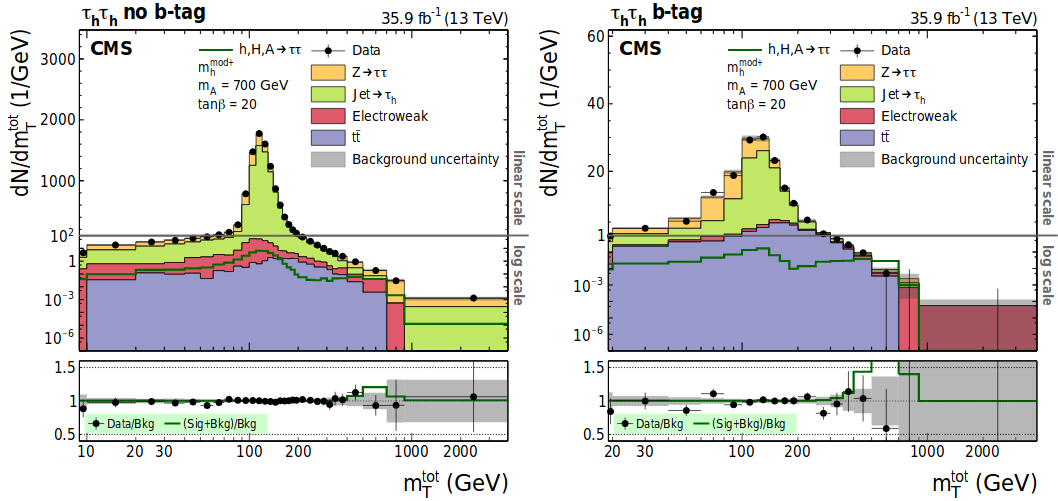
\includegraphics[width=\textwidth]{Images/2016MSSMmttot.png}
%     \caption{Distribution of \mttot in the global no b-tag (left) and b-tag (right) categories.}
%     \label{fig:control_plots}
% \end{figure}

A number of additional steps are needed to determine the \ma -  $\mathrm{tan}\beta$ limits. Signal samples are generated only for the set of \ma mass points to be tested, in the range $90$ to $3200$ GeV. The step size between points increases with \ma to scale with the worsening \mttot resolution. At each \ma -  $\mathrm{tan}\beta$ hypothesis, the masses of the other two Higgs bosons are calculated using results from the Higgs Working Group \cite{Dittmaier:1318996}. In each event category, templates for the h and H are generated by a horizontal morphing \cite{READ1999357} between templates from the two samples
closest in mass. The category acceptance is similarly interpolated from the neighbouring mass
points. All three templates are scaled by the appropriate cross sections and branching ratios and
combined into a single template. The $95\%$ CL upper limit is determined for each point on the \ma -  $\mathrm{tan}\beta$ grid, with the signal strength parameter $\mu$ uniformly scaling the entire signal model. The limit in  $\mathrm{tan}\beta$ is then defined as the point on which this upper limit is found to occur at $\mu = 1.0$. Practically, this is determined by interpolation between the points on either side of this threshold. Note that the SM Higgs boson is added to the background processes. This turns the likelihood ratio into a comparison between the MSSM and the SM Higgs sector hypotheses, and ensures a well defined problem even when the analysis becomes sensitive to the observed Higgs boson at $125\,\mathrm{GeV}$.

The observed and expected limits for the MSSM $m_{\mathrm{h}}^{\mathrm{mod}+}$ and the hMSSM scenarios are given in figure \ref{fig:limits}.

% \begin{figure}
%     \centering
%     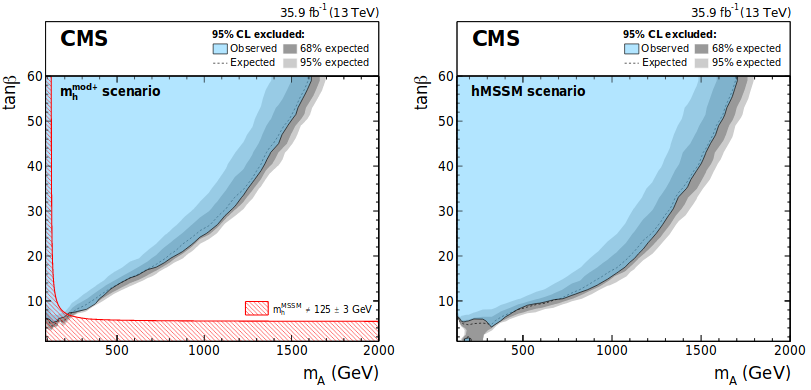
\includegraphics[width=\textwidth]{Images/MSSMlimits.png}
%     \caption{expected and observed $95\%$ CL exclusion contour (left) in the MSSM $m_{\mathrm{h}^{\mathrm{mod}+}}$ and (right) in the hMSSM scenarios. The expected median is shown as a dashed black line. The dark and bright gray bands indicate the 68 and 95 $\%$ confidence intervals for the variation of the expected exclusion. The observed exclusion contour is indicated by the coloured blue area. For the $m_{\mathrm{h}}^{\mathrm{mod}+}$ scenario, those parts of the parameter space, where $m_{\mathrm{h}}$ deviates by more than $\pm 3 \,\mathrm{GeV}$ from the mass of the observed Higgs boson at $125\,\mathrm{GeV}$ are indicated by a red hatched area.}
%     \label{fig:limits}
% \end{figure}

Figure \ref{fig:xslimits} gives model-independent upper limits on the production of a single neutral Higgs boson with mass $m_{\Phi}$. The limits on the cross section times branching fraction, $\sigma\times B(\Phi\rightarrow\tauh\tauh)$, are determined individually for gluon-gluon fusion and b-associated production. In the fit to extract gluon-gluon fusion limits the b-associated contribution is allowed to float freely, and vice versa. This is required as neither the no b-tag or b-tag categories are completely pure in one production mode, and this avoids the need to impose any assumptions about the ratio of cross sections between the two processes.

% \begin{figure}
%     \centering
%     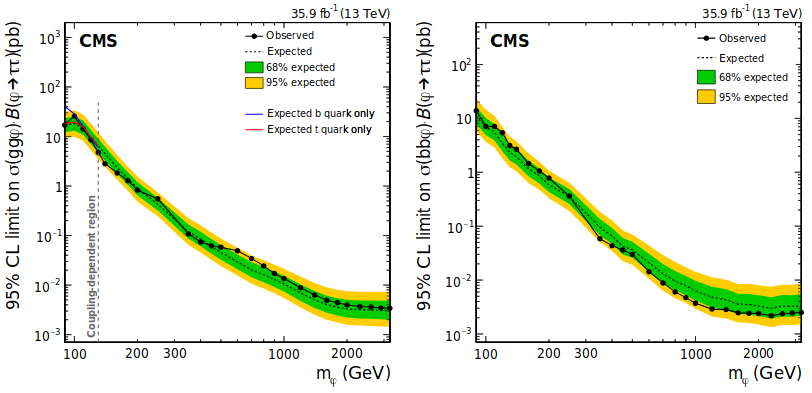
\includegraphics[width=\textwidth]{Images/xslimitsMSSM.png}
%     \caption{Expected and observed $95\%$ CL upper limits for the production of a single narrow resonance, $\Phi$, with a mass between $90\,\mathrm{GeV}$ and $3.2\,\mathrm{TeV}$ in the $\tauh\tauh$ final state (left) for the production via gluon fusion (gg$\Phi$ and (right) in association with b quark (bb$\Phi$). The expected median of the exclusion limit is shown by the dashed line. The dark green and bright yellow bands indicate the 68 and 95$\%$ confidence intervals for the variation of the expected exclusion limit. The black dots correspond to the observed limits.}
%     \label{fig:xslimits}
% \end{figure}

